\section{Benutzergruppen}

Zur Umsetzung des Rechtesystems von Roadrunner werden verschiedene Benutzergruppen eingeführt. Die Rechte werden einerseits direkt auf der Datenbank definiert und zudem noch über Validierungsfunktionen umgesetzt. Die Benutzerauthentifizierung wird von CouchDB durchgeführt.

\subsection{Admins \& Readers}

\begin{figure}
	\centering
		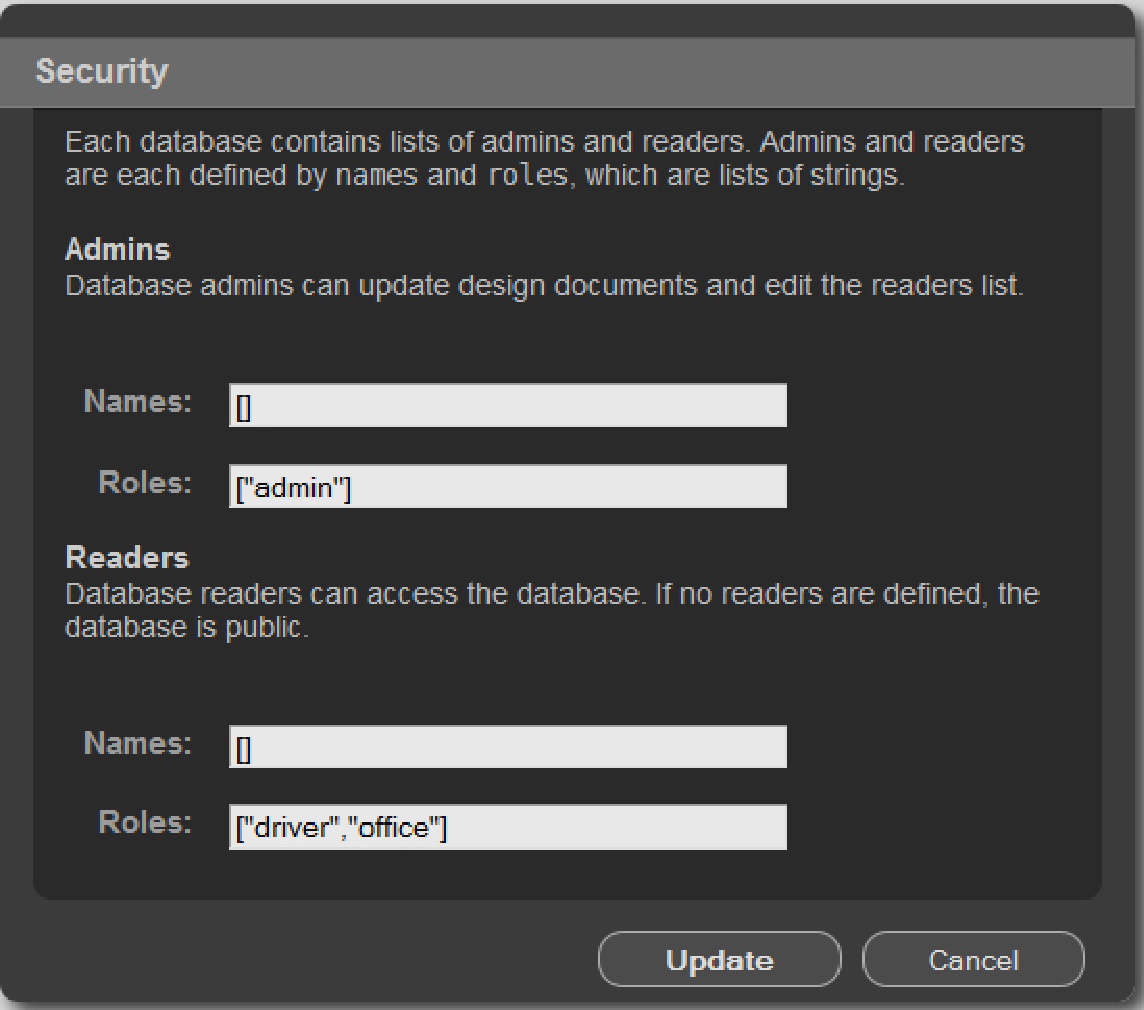
\includegraphics[width=0.8\textwidth]{files/pdf/security.pdf}
	\caption{Admins \& Readers}
	\label{fig:security}
\end{figure}

Auf einer Datenbank können in CouchDB Admins und Readers definiert werden. 
\begin{description}
\item[Admin] Ein Admin hat sämtliche Rechte auf der Datenbank. Er kann die zudem die Datenbank löschen, Designdokumente verändern oder Benutzerrechte ändern.
\item[Reader] Ein Reader hat lesenden und schreibenden Zugriff auf alle Dokumente bis auf die Designdokumente.
\end{description}

\noindent Ein Benutzer kann über 2 verschiedene Arten einer Gruppe zugeordnet werden:
 \begin{itemize}
\item Names: Ein CouchDB-Benutzer muss einen eindeutigen Namen im Format "`org.couchdb.user:[username]"' haben. Die Benutzer werden in einer seperaten Datenbank mit dem Namen "`\_users"' definiert. Wenn der Benutzer dieser Liste (Array aus Strings) hinzugefügt wird, dann besitzt er die entsprechenden Rechte.
\item Roles: Ein Benutzer kann verschiedene Rollen besitzen. Wenn eine seiner Rollen in dieser Liste aufgeführt wird, hat er die entsprechenden Rechte. 
\end{itemize}

\subsection{Rollen in Roadrunner}

Einem Benutzer können keine bis mehrere Rollen zugewiesen werden. Bei jeder Veränderung von Dokumenten auf dem Backendsystem wird von CouchDB eine Benutzerauthentifizierung durchgeführt. Bei dieser Benutzerauthentifizierung wird das Zugriffsrecht auf die Datenbank überprüft und zudem eine Validierung durchgeführt. Bei der Validierung werden alle definierten Validierungsmethoden aufgerufen. Nur wenn alle Validierungen gültig sind wird die gewünschte Änderung an den Dokumenten durchgeführt.
\newline \newline \noindent
Im Projekt Roadrunner wurden 3 verschiedenen Rollen definiert:
\begin{description}
\item[Admin] Ein Admin hat sämtliche Rechte auf der Datenbank. Diese Rollen ist ausschließlich für Administratoren vorgesehen.
\item[Office] Ein Benutzer der Gruppe Office arbeitet mit dem Backendsystem von Roadrunner. Dieser Benutzer arbeitet über die Webapplikation mit Roadrunner.
\item[Driver] Ein Benutzer der Gruppe Driver ist ein Fahrer. Er arbeitet auf dem Androidsystem mit Roadrunner. Auf dem Androidsystem arbeitet er als Admin mit der Datenbank. Eine Einschränkung der Benutzerrechte auf dem Androidsystem ist nicht nötig da die Benutzerauthentifizierung bei der Replizierung der Daten von dem Androidsystem auf das Backendsystem durchgeführt wird. Ein Fahrer kann nur Daten replizieren für die er die entsprechenden Rechte besitzt.
\end{description}

\noindent In den Validierungsmethoden werden die entpsrechenden Rechtevalidierungen durchgeführt. In Tabelle \ref{tab:rechte} sind die Berechtigungen aufgelistet. Ein + bedeutet, dass der Benutzer das Recht besitzt.

\begin{table}
\begin{tabular}{lccc}
& Driver & Office & Admin \\
Benutzerrechte ändern & - & - & + \\
Designdokumente ändern & - & - & + \\
Logeinträge anlegen & + & + & + \\
Logeinträge ändern & - & - & + \\
Logeinträge löschen & - & - & + \\
Andere Dokumente anlegen & - & + & + \\
Andere Dokumente ändern & - & + & + \\
Andere Dokumente löschen & - & + & +
\end{tabular}
\caption{Benutzerrechte}
\label{tab:rechte}
\end{table}